


\section{GloVe (Global Vectors for Word Representation)}


\begin{frame}{Problem With Word2Vec}
    
    \begin{itemizeSpaced}{0pt}
        \item \textbf{Problem: } Word2Vec uses local not global counts.  
        \begin{itemizeSpaced}{0pt}
            \item \textbf{Example: }``the" and ``cat" may occur frequently but Word2Vec does not know if this is because ``the" is a common word or because ``the" and ``cat" are actually correlated  (Kurita, 2018). 
            
        \end{itemizeSpaced}
        
        \item \textbf{Reason: } 
        \begin{itemizeSpaced}{0pt}
            \item Word2Vec implicitly optimizes over a co-occurrence matrix while streaming over input sentences $\Rightarrow$ context words are processed equally.
            
            \item Word2Vec's loss function $J = - \sum_i X_i \sum_j P_{ij} \text{log}(Q_{ij}) $ is the cross entropy between the \emph{predicted} and \emph{actual word distributions} in the context of word $i$.  \footnotemark 
            
            \item GloVe's authors say cross entropy models long-tailed distributions poorly, and here $X_i$ means equal-weighting over words. 
            
            \item Kurita (2018a) says there is no inherent justification for equal-streaming over words: GloVe uses \emph{unnormalized} probabilities. 
            
        \end{itemizeSpaced}
        
    \end{itemizeSpaced}
    
    \footnotetext[3]{\footnotesize $X_i = \sum_k X_{ik}$ is the total number of words appearing in the context of word $i$ \newline $Q_{ij} = \text{softmax} \Big( w_i \cdot w_j \Big)$ is the probability that word $j$ appears in context of word $i$}
\end{frame}




\begin{frame}{GloVe}

\begin{itemizeSpaced}{0pt}
    \item \textbf{Assumption: } words co-occur when they appear within a fixed sliding window $\Rightarrow$ reveals corpus-wide, not sentence-level word meaning.
\end{itemizeSpaced}

\begin{exampleBlock}{How GloVe Uses Co-Occurrence Ratios \footnotemark}
Consider two words $w_i =$ ``ice" and $w_j = $ ``steam". 

\begin{itemizeSpaced}{0pt}
    \item \textbf{Case 1:} For context words $\Tilde{w}_k$ related to ``ice" but not ``steam" ($\Tilde{w}_k = $ ``solid") $\Rightarrow$ expect co-occurrence probability $p_{\text{co}} \Big( \Tilde{w}_k \; | \; w_i \Big)$ is much larger than $p_{\text{co}} \Big( \Tilde{w}_k \; | \; w_j \Big)  \;\; \Rightarrow \;\; $ ratio $\frac {p_{\text{co}} \Big( \Tilde{w}_k \; | \; w_i \Big)} {p_{\text{co}} \Big( \Tilde{w}_k \; | \; w_j \Big)}$ gets very large.

    \item \textbf{Case 2: } Conversely, for words related to ``steam" but not ``ice" ($\Tilde{w}_k = $ ``gas") $\Rightarrow$ the co-occurrence ratio $\frac {p_{\text{co}} \Big( \Tilde{w}_k \; | \; w_i \Big)} {p_{\text{co}} \Big( \Tilde{w}_k \; | \; w_j \Big)}$ should be small. 

    \item \textbf{Case 3:} For $\Tilde{w}_k = $ ``water" related to both, or $\Tilde{w}_k = $ ``fashion" unrelated to either ``ice" or ``steam", then ratio $\frac {p_{\text{co}} \Big( \Tilde{w}_k \; | \; w_i \Big)} {p_{\text{co}} \Big( \Tilde{w}_k \; | \; w_j \Big)}$ is near one. 
\end{itemizeSpaced}
\end{exampleBlock}



\footnotetext[4]{GloVe defines word co-occurrence probability as: 
    $p_{\text{co}} \Big(w_k \; | \; w_i \Big) = \frac{C(w_i, w_k)}{C(w_i)}$  where $C(w_i, w_k)$ counts the co-occurrence between words $w_i$ and $w_k$.  }

\end{frame}



\begin{frame}{Performance: GloVe vs. Word2Vec}
    
    \cref{fig:gloveVsWord2vec} shows GloVe's learned embeddings have higher prediction accuracy over those of Skip-Gram and CBOW on \textbf{word analogy} and \textbf{named entity recognition (NER)}.
    
    \begin{figure}[h]
    \vspace{-5pt}
    \centering
    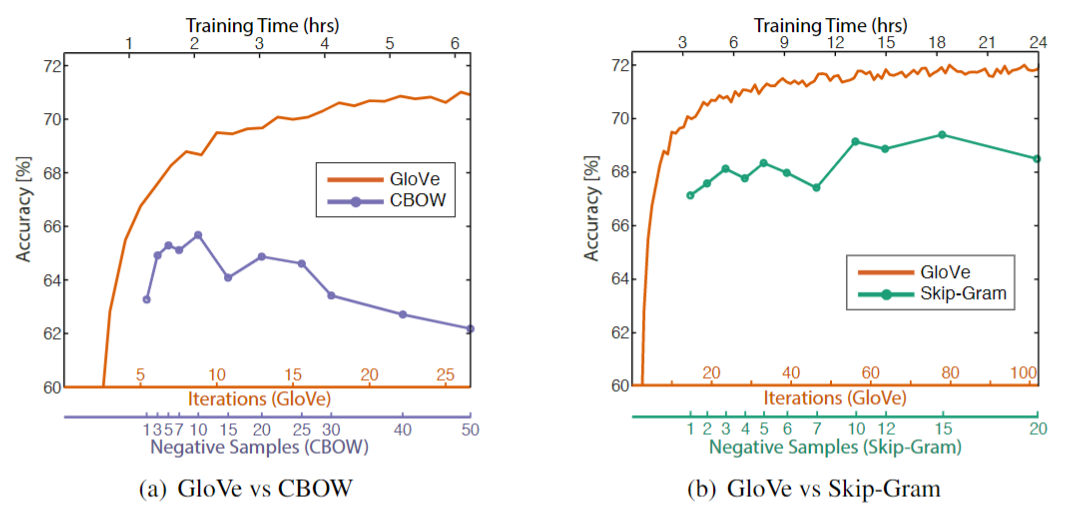
\includegraphics[width=0.99\textwidth]{imgs/table_gloveVSword2vec.png}
    \vspace{-5pt}
    \caption{\tiny Overall accuracy on word analogy task as a function of training time, which is governed by the number of iterations for GloVe and by the number of  negative samples for CBOW (a) and Skip-Gram (b). Pennington et al. (2014) train 300-dimensional vectors on the same 6B token corpus from Wikipedia and use a symmetric context window of size 10. From \emph{GloVe: Global Vectors for Word Representation}, by Pennington et al., 2014. \url{https://nlp.stanford.edu/pubs/glove.pdf}. Copyright 2014 by Pennington et al.}
    \vspace{-5pt}
    \label{fig:gloveVsWord2vec}
    \end{figure}
\end{frame}